\documentclass[conference,a4paper,10pt]{IEEETran}

\usepackage{amsmath,amssymb,amsfonts}
\usepackage{algorithmic}
\usepackage{graphicx}
\usepackage{textcomp}
\usepackage{xcolor}
\usepackage{multirow}
\usepackage{setspace}
\usepackage{pdfpages}
\usepackage{float}
\usepackage{caption,newfloat}
\usepackage[T1]{fontenc}
\usepackage[brazilian]{babel}
\usepackage[utf8]{inputenc}
\usepackage{ifthen}
\usepackage[pages=some]{background}
\RequirePackage[obeyspaces,hyphens]{url}
\RequirePackage[plainpages,pdfpagelabels]{hyperref}	% PDF com links, metadados
\RequirePackage{bookmark}				% cria um índice no PDF
\RequirePackage{microtype}	% melhorar a qualidade da tipografia no PDF


%% TODO
%% Se alguma hifenização não funcionar, adicionar aqui
\hyphenation{di-gi-ta-li-za-das}


%%%%%%%%%%%%%%%%%%%%%%%%%%%%%%%%%%%%%%%%%%%%%%%%%%%%%%%%%%%%%%%%%%%%%%%%
%     INÍCIO DO DOCUMENTO
%%%%%%%%%%%%%%%%%%%%%%%%%%%%%%%%%%%%%%%%%%%%%%%%%%%%%%%%%%%%%%%%%%%%%%%%
\begin{document}

%%%% NÃO MEXER NESTES ARQUIVOS
%%%% Definições/Estilos customizadas para o TADS, Mais capa
% \captionsetup{
%    tablename=TABELA,
%    listformat=empty,
%    justification=centering,
%    %labelsep=newline,
%    position=above,
%    skip=0.2\baselineskip,
%    width=\linewidth,
%    labelfont={small},
%    font={small} 
% }

\newcommand{\legenda}[1]{\caption{#1}}

\pagenumbering{arabic}

\def\BibTeX{{\rm B\kern-.05em{\sc i\kern-.025em b}\kern-.08em
    T\kern-.1667em\lower.7ex\hbox{E}\kern-.125emX}}

\newcommand{\tabelaname}{TABELA}
\newcommand{\figuraname}{FIGURA}
\newcommand{\quadroname}{QUADRO}
\newcounter{quadrocounter}
\setcounter{quadrocounter}{0}
% posicao, legenda, fonte
\newenvironment{quadro}[4][!t]
{
  \refstepcounter{quadrocounter}
  \label{#4}
  \def\fonteval{#3}
  \begin{table}[#1]
    \begin{center}
      % legenda
      \par\medskip\noindent
      QUADRO~\thequadrocounter~-~#2
      \par\medskip\noindent
}
{
      \par\noindent
      \fonte{\fonteval}
    \end{center}
  \end{table}
}
\newenvironment{quadro*}[4][!t]
{
  \refstepcounter{quadrocounter}
  \label{#4}
  \def\fonteval{#3}
  \begin{table*}[#1]
    \begin{center}
      % legenda
      \par\medskip\noindent
      QUADRO~\thequadrocounter~-~#2
      \par\medskip\noindent
}
{
      \par\noindent
      \fonte{\fonteval}
    \end{center}
  \end{table*}
}

\newcounter{tabelacounter}
\setcounter{tabelacounter}{0}
\newenvironment{tabela}[4][!t]
{
  \refstepcounter{tabelacounter}
  \label{#4}
  \def\fonteval{#3}
  \begin{table}[#1]
    \begin{center}
      % legenda
      \par\medskip\noindent
      TABELA~\thetabelacounter~-~#2
      \par\medskip\noindent
}
{
      \par\noindent
      \fonte{\fonteval}
    \end{center}
  \end{table}
}
\newenvironment{tabela*}[3][!t]
{
  \refstepcounter{tabelacounter}
  \def\fonteval{#3}
  \begin{table*}[#1]
    \begin{center}
      % legenda
      \par\medskip\noindent
      TABELA~\thetabelacounter~-~#2
      \par\medskip\noindent
}
{
      \par\noindent
      \fonte{\fonteval}
    \end{center}
  \end{table*}
}
\newcounter{figuracounter}
\setcounter{figuracounter}{0}
\newenvironment{figura}[4][!t]
{
  \def\fonteval{#3}
  \refstepcounter{figuracounter}
  \label{#4}
  \begin{figure}[#1]
    \begin{center}
      % legenda
      \par\medskip\noindent
      FIGURA~\thefiguracounter~-~#2
      \par\medskip\noindent
}
{
    \par\noindent
    \fonte{\fonteval}
    \end{center}
  \end{figure}
}
\newenvironment{figura*}[4][!t]
{
  \refstepcounter{figuracounter}
  \label{#4}
  \def\fonteval{#3}
  \begin{figure}[#1]
    \begin{center}
    % legenda
    \par\medskip\noindent
    FIGURA~\thefiguracounter~-~#2
    \par\medskip\noindent
}
{
    \par\noindent
    \fonte{\fonteval}
  \end{center}
  \end{figure}
}

\newcommand*{\captionsource}[2]{%
  \caption[{#1}]{%
  \centering
    #1%
    \hspace{\linewidth}%
    FONTE: #2%
  }%
}

\newcommand*{\fonte}[1]{%
  \centering
  \small
  \vspace{1em}
  \hspace{\linewidth}%
  FONTE: #1%
}

\def\abstractname{Abstract: }


%%%%%%%%%%%% CONFIGURAÇÃO DA CAPA E FOLHA DE ROSTO %%%%%%%%%%%%%%

\def\descr{Trabalho de conclusão de curso apresentado ao
curso de graduação em Análise e
Desenvolvimento de Sistemas, Setor de Educação
Profissional e Tecnológica, Universidade Federal
do Paraná, como requisito parcial à obtenção do
título de tecnólogo}



%%%% fundo na capa

\backgroundsetup{
scale=1,
color=black,
opacity=0.4,
angle=0,
contents={%
  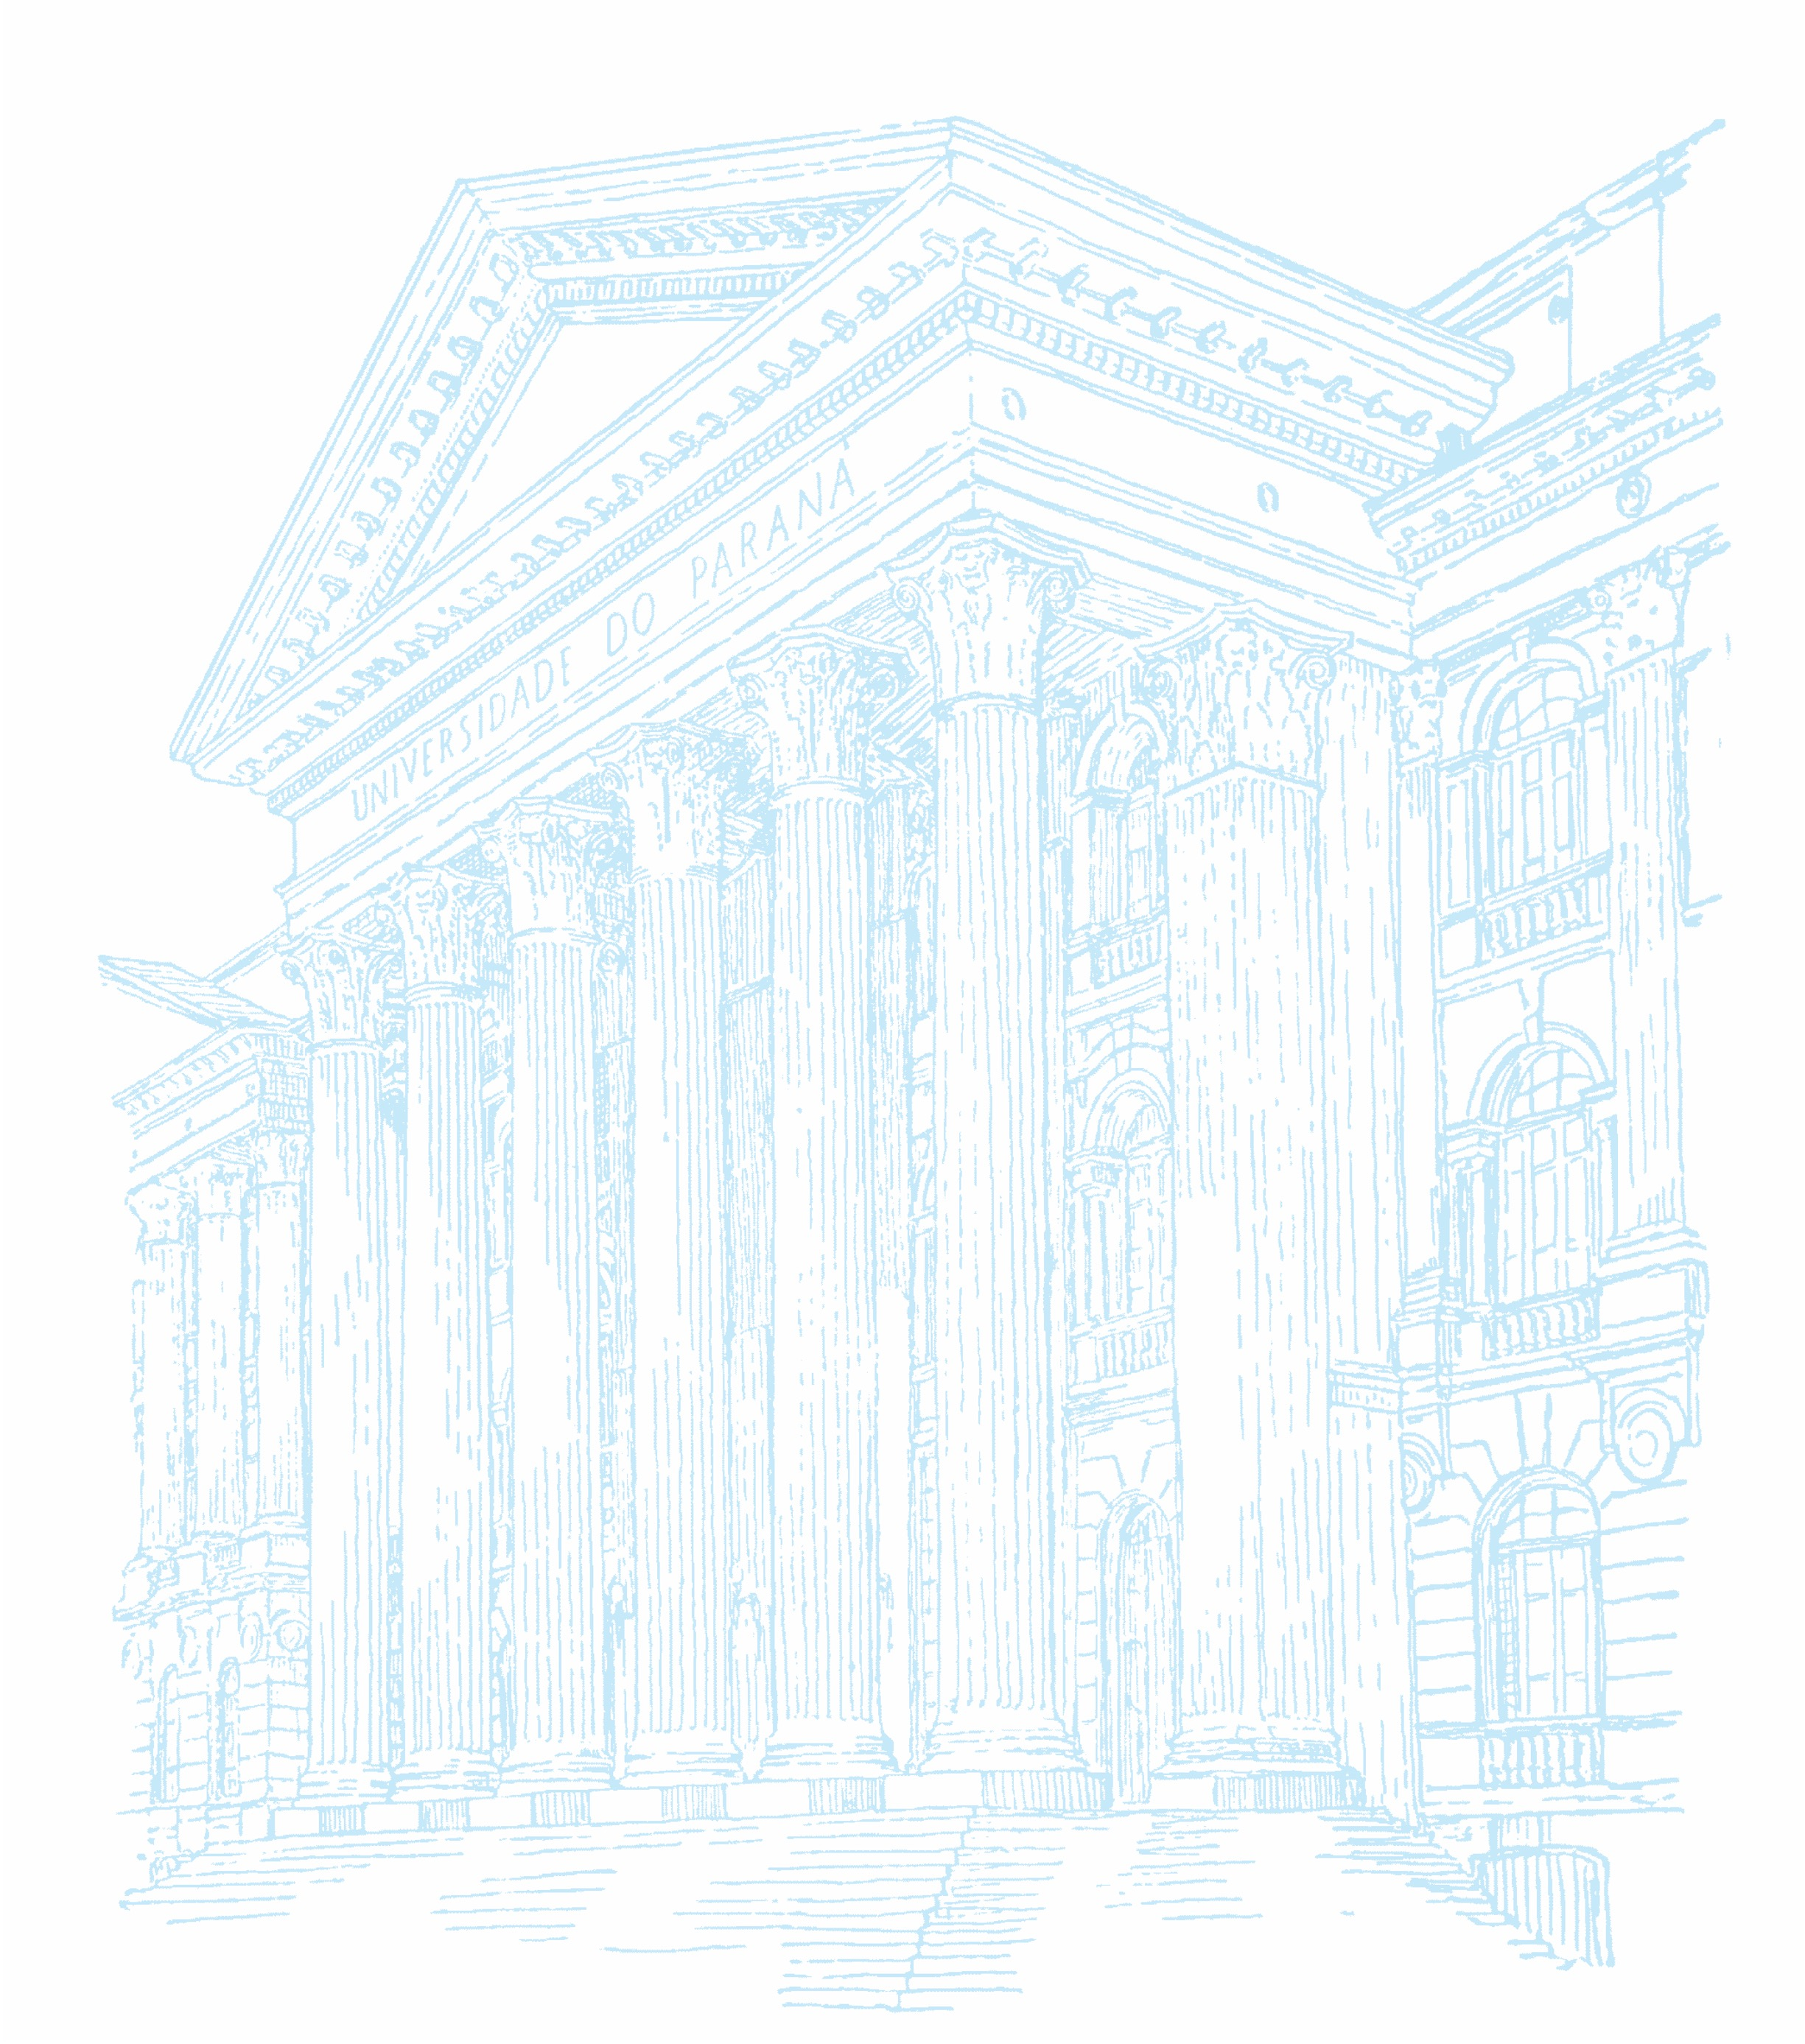
\includegraphics[width=\paperwidth,height=\paperheight]{bg_capa.jpg}
  }%
}
%%%%


%%%%%%% Definição da capa e folha de rosto


%\fancypagestyle{frontmatter}{
%  \fancyhf{}
%}

%\fancypagestyle{plain}{
%  \fancyhf{}
%  \if@mainmatter
%    \if@twoside
%      \fancyhead[LE,RO]{\thepage}
%    \else
%      \fancyhead[R]{\thepage}
%    \fi
%  \fi
%}



\hypersetup{
  % pdftitle, author, etc definidos mais abaixo
%  bookmarks   = true,
%  pageanchor  = false,
  hypertexnames = false,
%  bookmarkstype = page,
  pdfview     = Fit,
  pdfborder   = {0 0 0},
  colorlinks  = false,
  linkcolor   = blue,
  anchorcolor = blue,
  citecolor   = blue,
  filecolor   = blue,
%  pagecolor   = blue,
  urlcolor    = blue
}




%\def\@advisor{}			% orientador
%\def\@coadvisor{}		% co-orientador
%\def\@local{}			% local
%\def\@descr{}			% descrição do documento
%\def\@pcs{}			% palavras-chave
%\def\@kws{}			% keywords


%\newcommand{\autorcapa}[1]{\def\@author{#1}}
%\renewcommand{\title}[1]{\def\@title{#1}}

% descrição do documento na folha de rosto
%\newcommand{\descr}[1]{\def\@descr{#1}}

% orientadores
%\newcommand{\advisor}[1]{\def\@advisor{#1}}
%\newcommand{\coadvisor}[1]{\def\@coadvisor{#1}}


% local (cidade)
%\newcommand{\local}[1]{\def\@local{#1}}

\newcommand{\capa}[1]
{
  % páginas iniciais não são numeradas
  %\pagestyle{empty}
  %\thispagestyle{empty}

  % ajustar tags do PDF final
  \hypersetup{
    pdftitle    = {\titulo},
    pdfproducer = {UFPR - Universidade Federal do Paraná}
  }

  % primeira capa (só na versão aprovada)
  %\iffinalmode
%    \phantomsection
%    \thispagestyle{empty}

    \BgThispage
    
    \begin{center}
      \begin{doublespace}
        \textsc{\Large{UNIVERSIDADE FEDERAL DO PARANÁ}}
        \par
        \vspace{2cm}
        #1
        \vfill
        \DeclareRobustCommand\\{\linebreak}
        \textsc{\Large\titulo}
        \vfill
        \textsc{\Large\local\\\ano}
      \end{doublespace}
    \end{center}
    \cleardoublepage
    
    
  %\fi

  % folha de rosto
  \clearpage
%  \phantomsection
%  \addcontentsline{toc}{chapter}{Rosto}
%  \thispagestyle{empty}

  % autor
  \begin{center}
      \begin{doublespace}
        #1
      \end{doublespace}
  \end{center}

  \vfill\vfill

  % título
  \begin{doublespace}
    \begin{center}
      \DeclareRobustCommand\\{\linebreak }
      \textsc{\Large\titulo}
    \end{center}
  \end{doublespace}

  \vspace{1cm}

  % selo descritivo
  \hfill
  \begin{minipage}{9cm}

    % descrição
    \ifx\descr\@empty
    \else
      \descr.
    \fi

    % orientador
    \ifx\orientador\@empty
    \else
      \vspace{1em}
      Orientador: \orientadornome.
    \fi

    % coorientador
    \ifx\coorientador\undefined
    \else
      \vspace{1em}
      Co-orientador: \coorientador.
    \fi

  \end{minipage}

  \vfill

  % local e data
  \begin{center}
    \begin{doublespace}
      \textsc{\Large\local\\\ano}
    \end{doublespace}
  \end{center}

  % that's all, folks!
  \cleardoublepage
}


\newcommand{\termoaprovacao}
{
    \begin{center}
      \begin{doublespace}
        \vfill
        \Large{Substituir esta página pelo Termo de Aprovação que será fornecido após a defesa.}
        \vfill
      \end{doublespace}
    \end{center}
    \cleardoublepage
    
}

% \newcommand{\linebreakand}{%
%   \end{@IEEEauthorhalign}
%   \hfill\mbox{}\par
%   \mbox{}\hfill\begin{@IEEEauthorhalign}
% }

\newcommand*{\refmark}[1]{\raisebox{0pt}[0pt][0pt]{\textsuperscript{\footnotesize #1}}}
\newcommand{\autores}[1]{
  \author{
      \IEEEauthorblockN{
        #1
      }
      %\IEEEauthorblockN{#1\refmark{1}, #2\refmark{1}, #3\refmark{1}, #4\refmark{1}, #5\refmark{1}}
      \IEEEauthorblockA{\refmark{1}\textit{\setor} \\ \textit{\ufpr} }
  }
}

%%%%%%%



%%%%%%%%%%%%%%%%%%%%%%%%%%%%%%%%%%%%%%%%%%%%%%%%%%%%%%%%%%%%%%%%%%%%%%%%
%%%% Definições usadas para geração da capa, folha de rosto e títulos
%% TODO Alterar para seu trabalho
\def\autorescapa{
    \textsc{\Large GABRIEL VOLKOF MAYER}\\
    \textsc{\Large GUSTAVO SCHWANKA}\\
    \textsc{\Large LEONARDO XAVIER DA SILVA MORAES}\\
    \textsc{\Large LUCAS CASSILHA ZAWADNEAK}\\
    \textsc{\Large LUIS FELIPE FEZER}\\
}
\def\autorestitulo{
  Gabriel Volkof Mayer\refmark{1}, Gustavo Schwanka\refmark{1}, Lenoardo Xavier da Silva Moraes\refmark{1},\\
  Lucas Cassilha Zawadneak\refmark{1}, Luis Felipe Fezer\refmark{1}
}
\def\titulo{Sistema de Gerenciamento de Estágios no Ensino Superior}

\def\repositorio{https://bibliotecas.ufpr.br/}

\def\orientadornome{Profa. Dra. Rafaela Mantovani Fontana}
\def\orientadoremail{rafaela.fontana@ufpr.br}

% \def\coorientador{Profa. Dra. Rafaela Mantovani Fontana}

\def\local{Curitiba, PR}
\def\ano{2023}
\def\setor{Setor de Educação Profissional e Tecnológica}
\def\ufpr{Universidade Federal do Paraná}
\def\cidade{Curitiba, Brasil}
%%%%%%%%%%%%%%%%%%%%%%%%%%%%%%%%%%%%%%%%%%%%%%%%%%%%%%%%%%%%%%%%%%%%%%%%


%% Cria a capa em 1 coluna
\onecolumn

%%%%%%%%%%%%%%%%%%%%%%%%%%%%%%%%%%%%%%%%%%%%
% TODO : Adicionar o nome dos alunos aqui
\capa{\autorescapa}

%% Inclusão do Termo de Aprovação
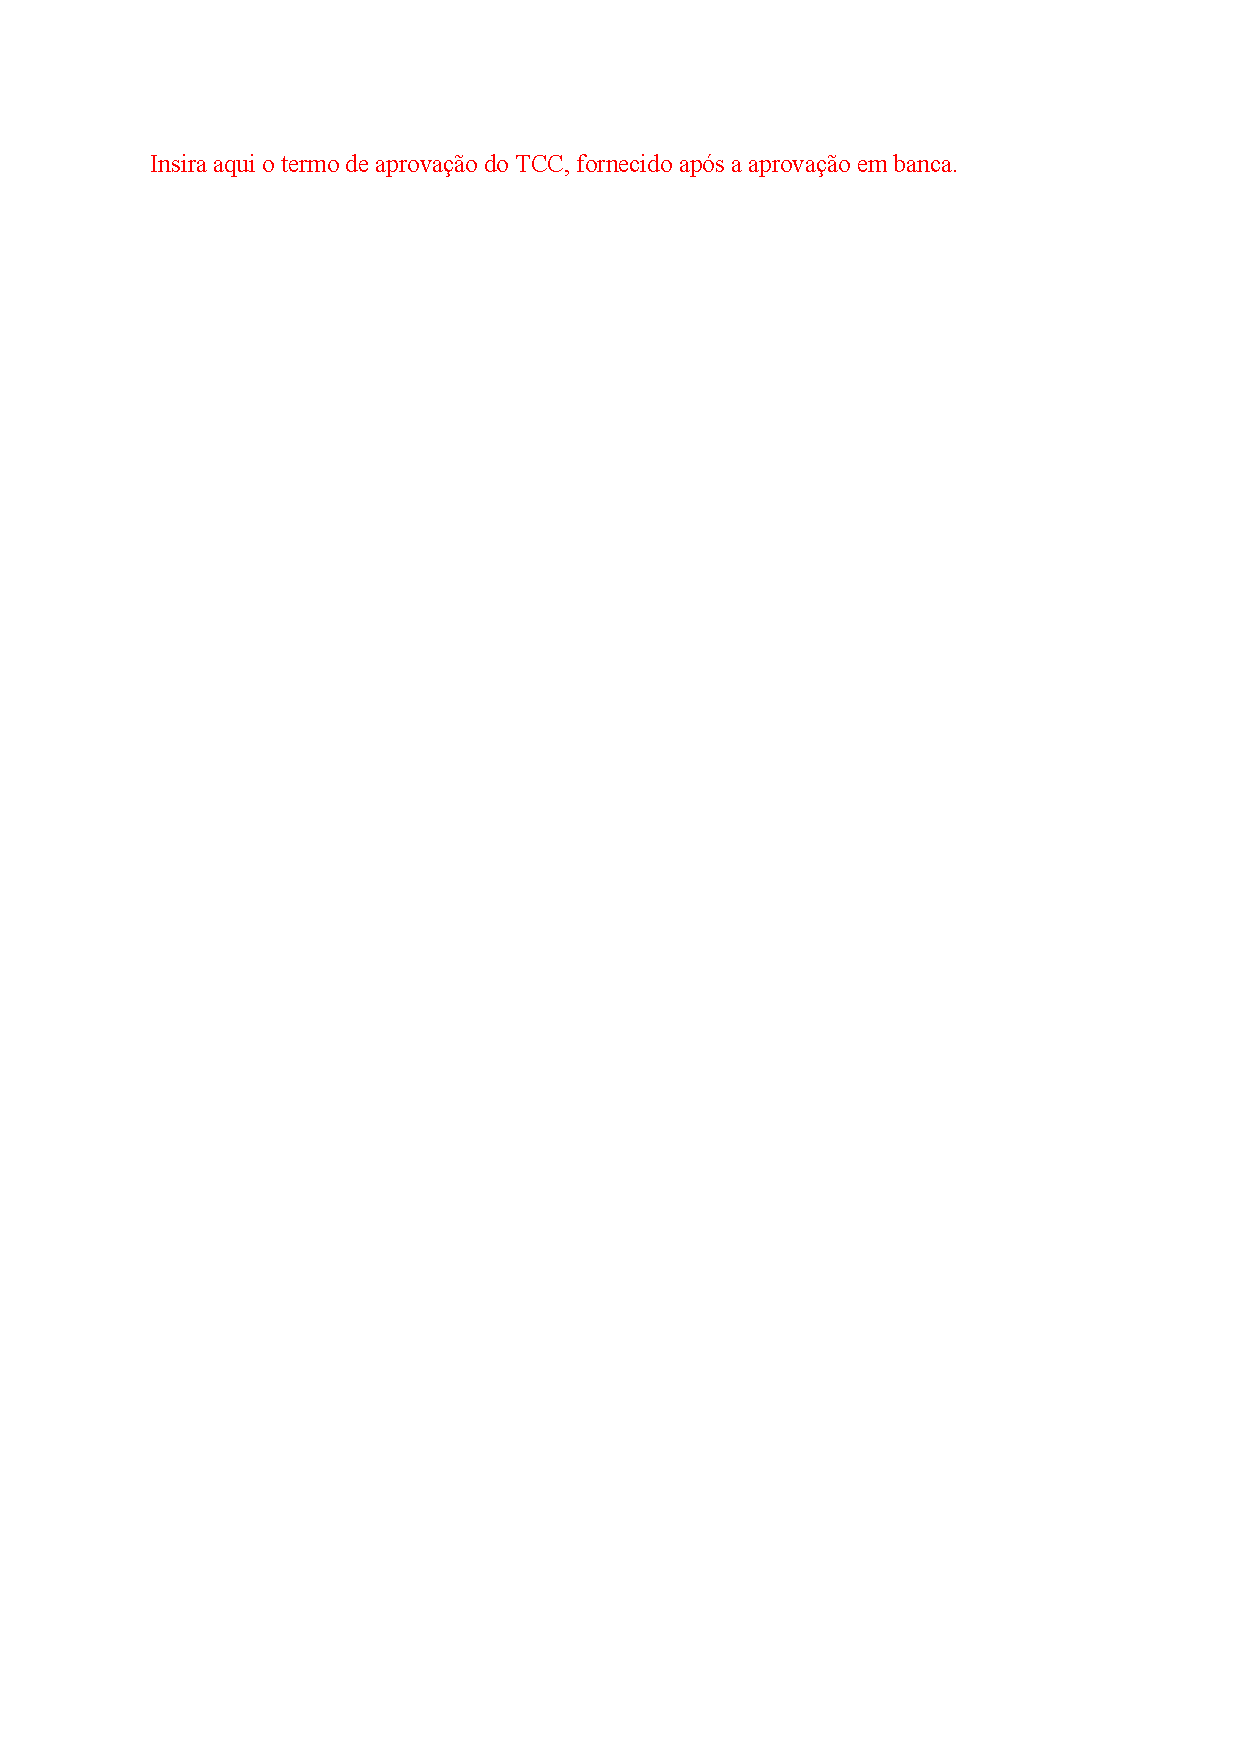
\includepdf{termo_aprovacao.pdf}

%% Cria o título do artigo
\twocolumn
\title{\titulo}

%%%%%%%%%%%%%%%%%%%%%%%%%%%%%%%%%%%%%%%%%%%%
\autores{\autorestitulo}

\maketitle

\thispagestyle{plain}
\pagestyle{plain}

%%%%%%%%%%%%%%%%%%%%%%%%%%%%%%%%%%%%%%%%%%%%%%%%%%%%%%%%%%%%
% Resumo e palavras-chave
\begin{resumo}
Este documento é um exemplo de artigo para o Trabalho de Conclusão de Curso (TCC) de Análise e Desenvolvimento de Sistemas da Universidade Federal do Paraná (UFPR). O conteúdo deste documento foi adaptado de um TCC já defendido no curso. O objetivo deste trabalho é definir e desenvolver um processo e um sistema que permitam a gestão dos estágios dos alunos da universidade. Sabe-se da importância do estágio  como atividade a ser desenvolvida pelo aluno, a fim de possibilitar que este tenha uma experiência em sua
área de estudo, garantindo que o conhecimento obtido no ambiente acadêmico seja colocado em prática no ambiente profissional. Em uma instituição como a UFPR, com um grande número de alunos realizando estágios, é imprescindível que a instituição possua formas automatizadas de conduzir o processo administrativo para realização do estágio e processos secundários, como termos aditivos e relatórios. O sistema foi desenvolvido seguindo as definições tecnológicas da Agência de Tecnologia da Informação e Comunicação (AGTIC): Java 17 com Spring Boot, Nuxt.JS, Sakai e MariaDB.
\end{resumo}

\begin{palavraschave}
Estágio; Sistema Integrado; SIGA; Módulo de Estágio.
\end{palavraschave}

%%%%%%%%%%%%%%%%%%%%%%%%%%%%%%%%%%%%%%%%%%%%%%%%%%%%%%%%%%%%
% Abstract e keywords
\begin{abstract}
This document is an example of a final paper (Trabalho de Conclusão de Curso – TCC) for the Systems Analysis and Development course at the Federal University of Paraná (UFPR). The content of this document was adapted from a TCC already defended in the course. The objective of this work is to define and develop a process and a system that enable the management of student internships at the university. The internship is known to be an essential activity for students, as it provides practical experience in their field of study, ensuring that the knowledge acquired in the academic environment is applied in the professional setting. At an institution such as UFPR, with a large number of students undertaking internships, it is crucial to have automated means to conduct the administrative process of managing internships, as well as related procedures such as amendments and reports. The system was developed in accordance with the technological guidelines of the Information and Communication Technology Agency (AGTIC), using Java 17 with Spring Boot, Nuxt.JS, Sakai, and MariaDB.
\end{abstract}

\begin{keywords}
Internship; Integrated System; SIGA; Internship Module.
\end{keywords}


%%%%%%%%%%%%%%%%%%%%%%%%%%%%%%%%%%%%%%%%%%%%%%%%%%%%%%%%%%%%
% Início do documento propriamente dito

\section{INTRODUÇÃO}

De acordo com a Resolução Nº 46/10 do Conselho de Ensino, Pesquisa e Extensão - CEPE\cite{ufpr_est_res}, que dispõe sobre os estágios na Universidade Federal do Paraná (UFPR), estágios são ``atos educativos escolares supervisionados que devem compor o projeto pedagógico dos cursos de graduação da UFPR'', ``atividades curriculares de base eminentemente pedagógica'' e ``atividades curriculares de caráter integrador''. Além da importância para o aluno, o estágio também possui seu valor para a universidade. A realização de um estágio significa que o aluno teve uma experiência profissional na área que deseja se formar, ou seja, é certo que foi propiciada uma oportunidade para aplicar os conhecimentos adquiridos no ambiente acadêmico. Ainda, a própria Resolução Nº 46/10-CEPE cita o estágio como atividade para o ``enriquecimento das destinações da UFPR (pesquisa, ensino e extensão) em sintonia com as necessidades tanto da comunidade próxima, como da vida nacional'' \cite{ufpr_est_res}. 

O processo para formalização de um estágio na UFPR passa por diferentes unidades, além do aluno: a Unidade de Estágios da Coordenação de Atividades Formativas e Estágios (UE/COAFE) da Pró-reitoria de Graduação e Educação Profissional (PROGRAD) é a responsável por gerenciar todos os estágios de estudantes da UFPR; A Comissão Orientadora de Estágio (COE) é vinculada ao colegiado de cada curso de graduação, sendo responsável pela aprovação dos estágios; o orientador, conforme Resolução nº 46/10-CEPE \cite{ufpr_est_res}, é um professor da UFPR responsável por acompanhar as atividades do estagiário do ponto de vista pedagógico; e o supervisor, externo à universidade, também é uma figura importante para o estágio, uma vez que é o profissional responsável pelo estagiário no local onde ele desenvolve suas atividades. Em alguns estágios, também há a presença do agente de integração – empresa privada que oferece vagas de estágio para seus clientes, muitas vezes sendo responsável pelo anúncio, além da gestão dos estagiários (como realização do acompanhamento de relatórios de estágio, por exemplo) \cite{ufpr_est_res}. 

Ao analisar o processo como ocorre atualmente, entendido a partir de entrevista com a PROGRAD\footnote{PROGRAD. Levantamento de Requisitos. Curitiba, 2022. Informação verbal - Entrevista}, nota-se que, do ponto de vista do aluno, três \textit{sites} diferentes devem ser acessados para que o processo de estágio seja aprovado, porém poderia ser feito em somente um. Ainda, analisando sob um ponto de vista administrativo, o processo também não ocorre de maneira ideal. Um formulário preenchido por um estudante no começo do processo só é computado no sistema quando um funcionário da instituição preenche um novo formulário, baseando-se no contrato com informações preenchidas pelo aluno. Em outras palavras, quando um estagiário preenche um formulário, este só é utilizado para gerar o contrato, ou seja, os dados não ficam salvos no sistema. Assim, evidencia-se a necessidade de integração do processo, facilitando a gestão.

O objetivo deste trabalho é, portanto, desenvolver um sistema capaz de tratar o fluxo
do processo de estágio de uma ponta à outra, isto é, desde o momento do preenchimento do formulário para gerar um termo de compromisso até a devolução do documento assinado para o aluno.

Neste contexto, este documento apresenta o relatório técnico da implementação deste sistema. A próxima seção apresenta a revisão de literatura os trabalhos semelhantes ao ao proposto, a Seção \ref{sec:mettecn} descreve o método de trabalho e as tecnologias utilizadas, a Seção \ref{sec:resultados} descreve a arquitetura do sistema e suas principais funcionalidades; e, por fim, a Seção \ref{sec:consfin} apresenta as considerações finais.

\section{REVISÃO DE LITERATURA}\label{sec:revlit}

Crucial para o desenvolvimento profissional dos estudantes brasileiros, o estágio é tratado juridicamente, no Brasil, desde o século XX. No período decorrido de lá até o presente momento, muito foi discutido sobre a legislação de estágio. Após diversas mudanças, pode-se, atualmente, dividir o estágio em duas formas, obrigatório e não obrigatório. Porém,
apesar dessa divisão, o objetivo é o mesmo: unir o conhecimento teórico, adquirido por meio dos estudos, ao conhecimento prático, a fim de possibilitar que o estagiário fique pronto para lidar com os desafios e obstáculos do dia a dia do trabalho, além de colocar em prática o conhecimento adquirido no ambiente acadêmico. Em sua primeira aparição jurídica no Brasil, o estágio foi definido como: 

\begin{quote}
``Um período de trabalho, realizado por aluno, sob o controle da competente autoridade docente, em um estabelecimento industrial [...]. Articular-se-á a direção dos estabelecimentos de ensino com os estabelecimentos industriais cujo trabalho se relacione com os seus cursos, para o fim de assegurar aos alunos a possibilidade de realização de estágios, sejam estes ou não obrigatórios.'' \cite[art.48]{brasil1942}
\end{quote}

Criada para dispor sobre o estágio dos estudantes, a lei nº 11.788, de 25 de setembro de 2008, também conhecida como Lei do Estágio \cite{brasil2008}, é a lei responsável por definir como deve ser um estágio no Brasil. A partir de sua sanção, duas grandes
mudanças passaram a ser previstas: de acordo com ela, o estagiário deve ter um tratamento diferenciado dentro da empresa e a instituição de ensino deve ser responsável por acompanhar e vincular o estágio ao processo didático-pedagógico formalmente. Ainda, conforme a Lei do Estágio:

\begin{quote}
``Estágio é ato educativo escolar supervisionado, desenvolvido no ambiente de trabalho, que visa à preparação para o trabalho produtivo de educandos que estejam frequentando o ensino regular em instituições de educação superior, de educação profissional, de ensino médio, da educação especial e dos anos finais do ensino fundamental, na modalidade profissional da educação de jovens e adultos.'' \cite[art.1o]{brasil2008}
\end{quote}

Na UFPR, a resolução Nº 46/10-CEPE \cite{ufpr_est_res} normatiza os estágios na instituição. De acordo esta resolução, ``A UFPR coordenará as atividades de estágios curriculares de caráter obrigatório, estendendo sua ação aos chamados estágios não obrigatórios [...]'', com duração mínima de um período letivo. Ainda, há outros artigos tratando de outros assuntos relacionados ao estágio, como campo de estágio, a orientação, a supervisão, a administração, entre outros.

Ainda, há a Instrução normativa Nº 01/12-CEPE \cite{ufpr_est_in}, que normatiza os estágios curriculares não obrigatórios, previstos na resolução nº 46/10-CEPE, complementada por uma outra série de instruções normativas que definem os detalhes do processo de administração dos vários tipos de estágio que podem ser realizados na instituição.

\subsection{Processo de gestão de estágio na UFPR}

Atualmente, conforme apurado em entrevista com a PROGRAD, a UFPR não desfruta de um sistema voltado especificamente para o processo de gestão de estágios. Assim, quando um estudante deseja passar pelo processo de estágio, o seguinte fluxo ocorre (em caso de aprovação):

\begin{itemize}
    \item O estudante acessa um site, cuja única finalidade é disponibilizar formulários referentes ao estágio;
    \item O estudante escolhe o formulário desejado, preenche e baixa um documento em formato Portable Document Format (PDF) do contrato
gerado após o formulário ser submetido;
    \item O contrato gerado por meio do site deve ser assinado pelo estudante e enviado à parte concedente para que esta assine;
    \item Após o estudante e a parte concedente terem assinado, o aluno deve procurar o professor orientador para coletar sua assinatura;
    \item Em seguida, com as três assinaturas, deve ser realizado um \textit{upload} do contrato na Secretaria On-line ou no SEI, a depender do campus do curso do aluno;
    \item Disponibilizado na Secretaria Online, o contrato segue para análise da COE, coordenação e COAFE, responsáveis pela aprovação ou rejeição do processo;
    \item Ao término da análise, o contrato é retornado ao estudante via e-mail.
\end{itemize}

\subsection{Trabalhos semelhantes}\label{sec:trabsem}

Somente um sistema efetivamente semelhante ao que este trabalho propõe foi encontrado, trata-se do Sistema HDE \cite{sistemahde}. Por ser pago, não foi possível obter acesso ao software, porém sabe-se que cumpre o propósito de gerenciar estágios, suportando o aluno e a instituição de ensino. O sistema oferece uma solução tanto para um agente de integração quanto para uma instituição de ensino. De acordo com o encontrado no portal da organização, o sistema possibilita:

\begin{quote}
``Atuar com ou como Agentes de Integração, acompanhar a gestão de estágio ou simplesmente promover a Empregabilidade! Sim, pode-se escolher o
papel com o qual se deseja atuar, e podemos te mostrar como, abrir os horizontes e ainda buscar fechar o ciclo que se inicia quando um estudante inicia seu curso e finaliza com este inserido no mercado de trabalho'' \cite{sistemahde}.
\end{quote}

Ainda de acordo com o próprio portal do Sistema HDE \cite{sistemahde}, benefícios como integração com o sistema acadêmico utilizado, vagas de estágio para os estudantes da universidade e gestão de contratos de estágio são citados como benefícios às instituições de ensino.
Outros softwares gerenciadores de estágio foram encontrados, mas focam somente na parte concedente, fugindo da intenção deste projeto.

\section{MÉTODO E TECNOLOGIAS} \label{sec:mettecn}

A fim de desenvolver este trabalho, estudou-se o processo do fluxo de estágios na Universidade Federal do Paraná. Para isso, realizaram-se pesquisas e entrevistas com pessoas e entidades envolvidas diretamente com o processo. Possibilitou-se, assim, um maior entendimento do processo e dos problemas nele presentes. A partir do conhecimento do processo como um todo, pôde-se desenvolver um sistema como solução para os problemas encontrados.

O modelo de engenharia de software escolhido para conduzir o processo de desenvolvimento foi o Scrum \cite{schwaber2020}. Parte fundamental do Scrum, a \textit{sprint} representa uma iteração e é composta por quatro eventos principais. A reunião de planejamento da \textit{sprint} marca seu início e tem como objetivo estabelecer o trabalho a ser realizado durante a iteração. A scrum diária, com duração máxima de 15 minutos, busca alinhar o progresso em direção ao objetivo da sprint e adaptar o \textit{backlog} conforme necessário; nela, cada membro da equipe deve responder o que foi feito desde a última reunião, o que pretende realizar até a próxima e se há algum impedimento para a execução das tarefas. A revisão da \textit{sprint} visa inspecionar os resultados obtidos e determinar possíveis adaptações para aprimorar o produto. Por fim, a retrospectiva da \textit{sprint} é realizada com o propósito de planejar estratégias que aumentem a qualidade e a eficácia do processo. \cite{schwaber2020}. Complementarmente ao Scrum, a abordagem Kanban foi utilizada para organização e acompanhamento das tarefas realizadas pela equipe \cite{gross2003}.

O desenvolvimento do projeto foi dividido em duas grandes etapas: modelagem e desenvolvimento. Na
primeira etapa, voltada à modelagem, houve a elicitação de requisitos, o desenvolvimento dos Protótipos de Telas, do Diagrama macro representativo do fluxo de um termo de compromisso de estágio, do Diagrama de Classes, das Histórias de Usuário, do Diagrama de Casos de Uso, do Diagrama Lógico-Relacional do Banco de Dados, dos Diagramas de Sequência  e do Diagrama de Processo de Negócio. A notação dos modelos foi a definida pela \textit{Unified Modeling Language} (UML). Na modelagem as sprints do Scrum tiveram duração de uma semana.

A Figura ~\ref{fig:diagcasosdeuso} apresenta um exemplo de um dos diagramas de casos de uso criados para o projeto - relativo ao Cadastro do Termo de Compromisso de Estágio. A documentação completa pode ser encontrada no acervo da Biblioteca da UFPR \footnote{https://bibliotecas.ufpr.br/}. 

Já na segunda etapa do projeto - que foi o desenvolvimento do sistema - as tecnologias descritas a seguir foram empregadas com a finalidade de implementar as funcionalidades definidas na etapa de modelagem, resultando na implementação do sistema conforme a arquitetura descrita na Seção ~\ref{sec:resultados}. Ao longo do desenvolvimento, as sprints tiveram duração de duas semanas, para que a equipe pudesse produzir histórias de usuário completas. O código-fonte do sistema também pode ser encontrado no acervo da Biblioteca da UFPR \footnote{https://bibliotecas.ufpr.br/}. 

\begin{figura}[htbp]{Exemplo de Diagrama de Casos de Uso - Cadastrar Termo de Compromisso de Estágio.}{Os autores (2023)}{fig:diagcasosdeuso}
  \centerline{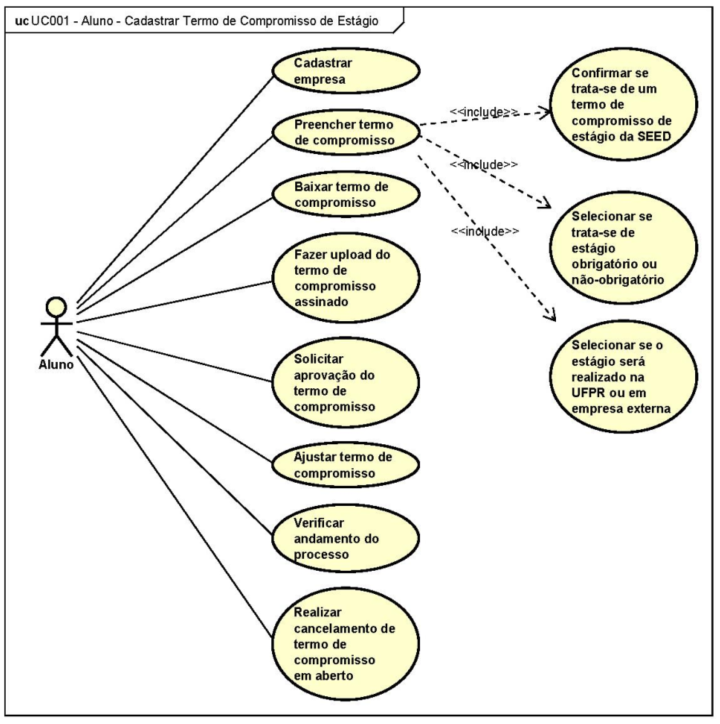
\includegraphics[width=0.45\textwidth]{diag_casos_uso.png}}
\end{figura}

A documentação do sistema contempla, também, as histórias de usuário criadas para o projeto. Cada diagrama de caso de uso foi definido com um épico, que, por sua vez, desdobrou-se em um conjunto de história de usuário no formato <SENDO><QUERO><PARA>.

Com relação às tecnologias utilizadas para o desenvolvimento, adotou-se um conjunto de ferramentas indicadas pela Agência de Tecnologia da Informação e Comunicação (AGTIC), de forma que o sofwtare resultante pudesse ser facilmente absorvido pela estrutura já disponível na UFPR. O \textit{frontend} foi desenvolvido com uma estrutura baseada em Java Script, enquanto o \textit{backend} foi construído sobre uma estrutura baseada em Java. A Tabela~\ref{tabtecnologias} detalha e descreve brevemente as tecnologias empregadas. 

\begin{tabela}[t!]{Tecnologias Utilizadas.}{Os autores (2023)}{tabtecnologias}
  \begin{tabular}{c|l}
    \hline
    \textbf{Tecnologia}&\textbf{Utilização}\\
    \hline
    Nuxt          & Framework de \textit{frontend} \cite{nuxt2023} \\
    Sakai         & Template de estilos \textit{frontend}\cite{bhowmik2022}\\
    Java          & Desenvolvimento do \textit{Backend} \cite{oracle2023}\\
    Spring Boot   & Framework de desenvolvimento \textit{backend} \cite{spring2023}\\
    Maria DB      & Banco de dados \cite{mariadb2023} \\
    Keycolak      & Gerenciamento de identidade e acesso \cite{keycloak2023} \\
    Git           & Controle de versão e código \cite{git2023}\\
    \hline
  \end{tabular}
\end{tabela}

\section{RESULTADOS} \label{sec:resultados}

Este capítulo tem como objetivo apresentar o sistema desenvolvido: sua arquitetura e as suas principais funcionalidades.

\subsection{Arquitetura do Sistema}

A arquitetura geral do sistema é representada pela Figura ~\ref{fig:arquitetura}. Conforme apresentado na Tabela ~\ref{tabtecnologias}, a arquitetura foi baseada em tecnologias atuais e amplamente utilizadas, como Nuxt, Spring Boot e MariaDB. O sistema foi criado, também, com uma integração com o SIGA.

O SIGA é responsável pelo gerenciamento dos dados de todos os alunos da UFPR. É por ele que são realizadas a disponibilização de turmas para matrícula, construção da grade horária pelos alunos, emissão de documentos, entre outros processos gerais. É a partir do SIGA que são disponibilizados dados importantes para o módulo de estágio desenvolvido neste projeto, como dados do aluno, matrícula e professores. Estas informações ficam no banco de dados principal do SIGA, e são acessados pelo backend do módulo de estágios somente quando necessário.

\begin{figura}[htbp]{Representação da arquitetura do sistema.}{Os autores (2023)}{fig:arquitetura}
  \centerline{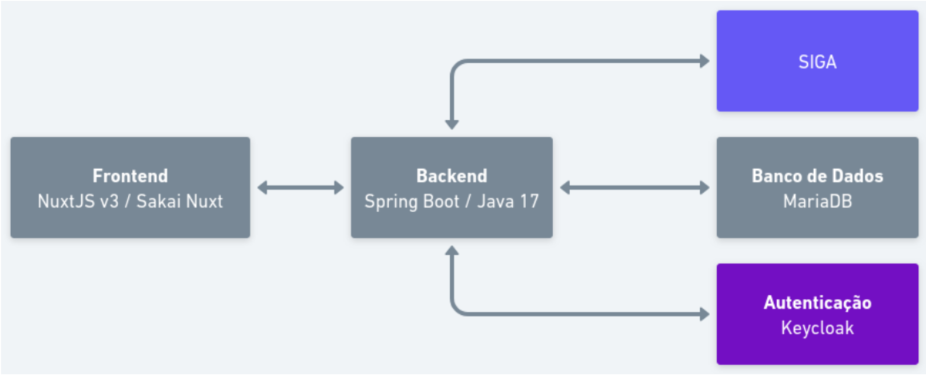
\includegraphics[width=0.45\textwidth]{arquitetura.png}}
\end{figura}

Na Figura ~\ref{fig:arquitetura} observa-se o \textit{frontend} - que é a parte que o usuário acessa e utiliza para gerenciar suas informações e processos de estágio; o \textit{backend} - responsável por gerir todas as regras de negócio do sistema, e suprir o \textit{frontend} com os dados do sistema e o banco de dados, que armazena as informações referentes a todos os processos e dados do módulo. Observa-se, também, a utilização do KeyCloak - responsável por gerenciar o acesso dos usuários. As informações referentes aos alunos e docentes da UFPR são disponibilizadas pela API (\textit{Application Programming Interface}) do SIGA.

\subsubsection {Integração com o SIGA}

A integração com o SIGA é feita de modo que não seja necessário acessar ou alterar qualquer código interno do sistema atual por parte da equipe do módulo de estágios. Todo o código de acesso externo à API do SIGA é mantido pela equipe que mantém o SIGA atualmente. Isso faz com que, para o módulo de estágios, apenas o necessário seja acessado, sem precisar fazer uma análise profunda da estrutura do SIGA.

Essa integração é feita de forma que seja necessário somente realizar requisições para a API disponibilizada pela Universidade, que retorna dados pontuais e específicos de cada caso. Um exemplo disso se dá durante a criação de um termo de compromisso por parte de um aluno, onde é necessário escolher o professor orientador. Nesse momento, a API do SIGA é consumida para buscar os dados de todos os professores do curso do aluno, e tal informação é disponibilizada para seleção do usuário.

Em paralelo a essa integração, também foram desenvolvidos o \textit{frontend} e o \textit{backend} do projeto do módulo de estágios. Ambas as partes foram inteiramente desenvolvidas pela equipe, tendo como parâmetros as definições arquiteturais definidas pela AGTIC, para que este projeto possa ser absorvido pela UFPR no futuro.

\subsection{Apresentação do Sistema}

O sistema foi desenvolvido com a finalidade de centralizar as responsabilidades do aluno, COAFE, COE e coordenação acerca do processo do estágio. Para isso, além das funcionalidades já existentes, como cadastrar estágio, por exemplo, houve a inclusão de novos recursos.

O ator aluno é o responsável por dar início ao processo: após fazer login para entrar no sistema, o início do processo se dá pelo preenchimento de um formulário para gerar um termo de compromisso de estágio, confome mostra a tela da Figura ~\ref{fig:novo_termo}. Neste momento, o aluno seleciona qual é o tipo de estágio que será realizado: obrigatório ou não obrigatório, na UFPR ou em empresa externa. Depois, preenche todas as informações pertinentes ao estágio e, em seguida, gera um documento em formato PDF.

Com o documento gerado, mas agora de maneira externa ao sistema, o aluno é responsável por coletar
a assinatura do professor orientador e do supervisor do estágio. Com as assinaturas coletadas, o aluno deve retornar ao sistema e realizar o \textit{upload} do documento. A seguir, o próximo passo do aluno é solicitar a aprovação do documento.

Além do termo de compromisso de estágio, o ator aluno também pode utilizar o sistema para emissão de outros documentos, como o termo aditivo, o termo de rescisão, a ficha de avaliação e o relatório de estágio, bem como realizar a solicitação de certificado de estágio, caso o estágio realizado tenha sido do tipo não obrigatório. Ainda, o aluno pode baixar os documentos que foram submetidos por ele próprio, cancelar processos e atualizar alguns dos seus dados. 

O ator COE só possui ação em estágios não obrigatórios. No caso do termo de compromisso de estágio, a COE tem a possibilidade de listar os termos pendentes de aprovação, termos indeferidos, termos cancelados, termos em análise por outros atores, bem como baixar um termo submetido por um aluno. Essas funcionalidades
permitem o indeferimento, solicitação de ajustes no termo e a aprovação. Para os outros termos de estágio, a COE possui as mesmas funcionalidades de listar, aprovar, indeferir e solicitar ajustes.

O ator COAFE, ao contrário da COE, atua em todos os tipos de estágios. No entanto, diversas funcionalidades são parecidas, como listar processos indeferidos, pendentes de aprovação, cancelados ou em análise por outros atores, com a diferença sendo composta pela possibilidade de filtrar pelo tipo de estágio (obrigatório
ou não obrigatório). Outra diferença entre a COE e a COAFE é que esta pode gerar relatórios em formatos PDF e xlsx para contratante, agente integrador, certificados de estágio, relatórios de estágio e estágios com a seguradora UFPR. As necessidades de tais relatórios se deram a partir de uma entrevista com os membros da COAFE, os quais indicaram que tal possibilidade seria de grande proveito para o trabalho deles. 

O ator coordenador possui papel crucial nos fluxos de estágio. Para que um aluno comece um estágio, por exemplo, este ator, a partir do sistema, deve dar ciência na formação do supervisor, no plano de atividades e no Índice de Rendimento Acadêmico (IRA) do aluno. Caso um termo de compromisso seja indeferido, o coordenador também deve dar ciência no indeferimento. Ainda, o coordenador também pode listar, aprovar e baixar documentos de alunos de um curso coordenado por ele. 

Por último, o ator orientador também pode listar os documentos, além de dar ciência no relatório de estágio e no termo de rescisão. Há, também, a possibilidade de gerar certificado de estágio para cada estágio não obrigatório orientado por ele.

Quando o estágio inicia, o aluno possui uma tela específica (Figura ~\ref{fig:estagio_ativo}) no sistema que permite todas as ações obre um estágio ativo, como inclusão de um termo aditivio, rescisão, entre outras. 

\begin{figura}[htbp]{Tela para criação de um novo termo de estágio.}{Os autores (2023)}{fig:novo_termo}
  \centerline{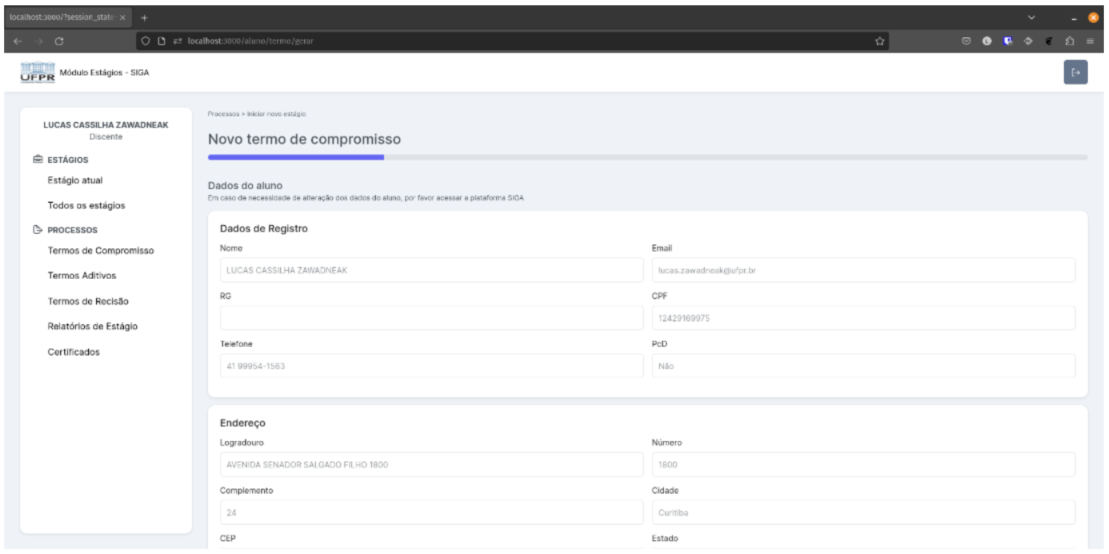
\includegraphics[width=0.45\textwidth]{novo_termo.PNG}}
\end{figura}

\begin{figura}[htbp]{Tela de estágio ativo.}{Os autores (2023)}{fig:estagio_ativo}
  \centerline{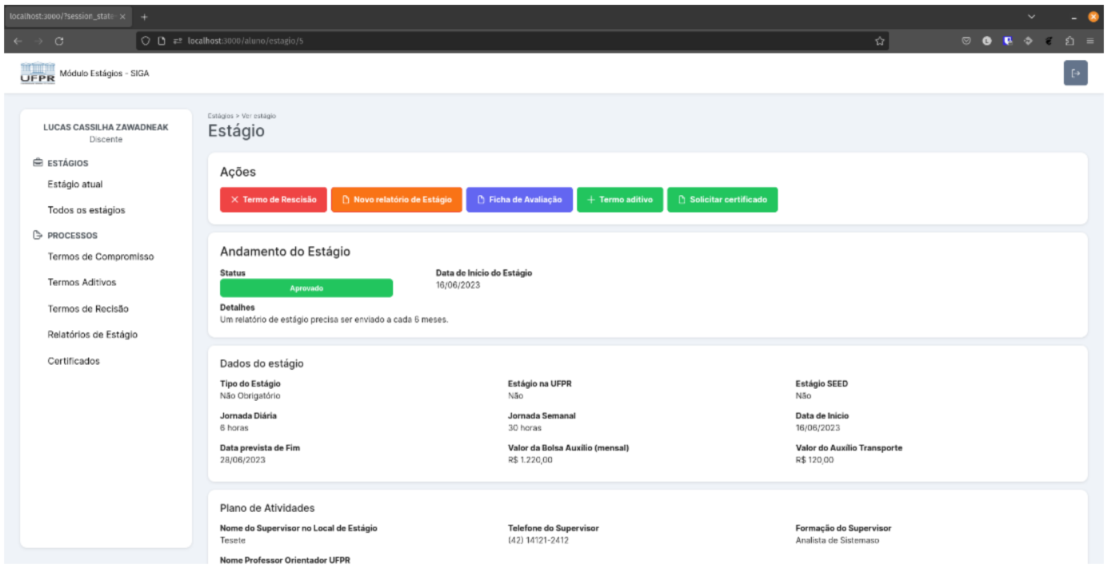
\includegraphics[width=0.45\textwidth]{estagio_ativo.PNG}}
\end{figura}

\section{CONSIDERAÇÕES FINAIS} \label{sec:consfin}

O estágio é importante para a formação acadêmica de um aluno, uma vez que proporciona a oportunidade de colocar em prática os conhecimentos adquiridos no ambiente acadêmico e de adquirir novas habilidades e experiências. Por meio do estágio, os alunos têm uma visão mais ampla do mercado de trabalho, além de obter uma experiência na sua área, o que possibilita novas oportunidades para o seguimento da carreira.

Um sistema integrado de gerenciamento de estágios para universidades proporciona aos coordenadores e professores responsáveis pelos estágios uma maior praticidade ao acompanhar os processos dos alunos, facilitando a visualização dos
processos em aberto que dependam de suas aprovações. Ainda, um sistema integrado possibilita um maior controle macro por parte da parte administrativa, uma vez que terá o acesso facilitado a relatórios.

O objetivo deste trabalho foi, portanto, o desenvolvimento de um sistema de estágios integrado ao sistema de gestão acadêmica (SIGA) da UFPR. O método de trabalho utilizou o Scrum como modelo de processo de engenharia de software, a UML como linguagem de modelagem do sistema e as tecnologias Java 17 com Spring Boot, Nuxt.JS, Sakai e MariaDB para desenvolvimento de sistema.

Resultando, desta forma, em um sistema capaz de tratar o fluxo do processo de estágio de uma ponta à outra, isto é, desde o momento do preenchimento do formulário para gerar um termo de compromisso de estágio até a devolução do termo aprovado para o aluno, bem como a informatização de outros fluxos associados ao processo de estágio, como: fluxo do termo aditivo, fluxo do termo de rescisão, fluxo de relatório de estágio, dentre outros.
 
Evidenciou-se, portanto, que o desenvolvimento de um sistema integrado de estágios é fundamental para garantir a eficiência e a qualidade do processo de estágio, contribuindo para a formação acadêmica e profissional dos alunos. Assim,
este trabalho, além de implementar um sistema que permite o controle do processo de estágio, também pôde contribuir com a UFPR, uma vez que se identificou a possibilidade de integrá-lo como um serviço ao SIGA e, em decorrência disso,
optou-se pelas tecnologias utilizadas por tal sistema.

\subsection{Recomendações para trabalhos futuros} 
Diversas são as possibilidades para trabalhos futuros. No entanto, destaca-se a implementação de um sistema de assinaturas também no SIGA, uma vez que possibilitaria uma maior praticidade aos futuros estagiários e aos atores envolvidos na
parte administrativa da UFPR. Em caso de sucesso na implementação deste projeto como serviço no SIGA, abrir-se-á um leque de possibilidades de colaboração das atividades acadêmicas com as necessidades administrativas da universidade, uma vez que este trabalho poderá servir como exemplo para projetos de tecnologia da informação.


\section{Artefatos}

Os artefatos de modelagem e código-fonte desenvolvidos estão disponibilizados no acervo da Biblioteca da UFPR: \texttt{\repositorio}.


%%%%%%%%%%%%%%%%%%%%%%%%%%%%%%%%%%%%%%%%%%%%%%%%%%%%%%%%%%%%
% REFERÊNCIAS

\def\refname{Referências}

\bibliographystyle{abntex2-num}
\bibliography{referencias}



\end{document}
